\section{Network Management, SNMP e NETCONF}

Una rete di calcolatori è un sistema intrinsecamente complesso, con
migliaia di componenti hardware e software che interagiscono tra loro. 
Questa complessità rende la gestione
attiva della rete non solo un'esigenza tecnica ma un requisito strategico
fondamentale per garantire l'efficienza, l'affidabilità e la qualità del
servizio (QoS).

Il \textbf{Network Management (NM)} è quindi l'insieme di attività di deployment, 
integrazione e coordinamento degli elementi hardware, software e umani per monitorare, 
testare, interrogare, configurare, analizzare, valutare e controllare la rete e le sue
risorse. L'obiettivo finale è ottimizzare le prestazioni e la QoS a un costo
ragionevole, considerando il costo totale che include non solo il traffico dati
ma anche il consumo energetico e delle risorse. Nel NM si vuole al più possibile
limitare l'intervento umano, affidandosi a sistemi automatizzati e intelligenti.

Le attività di gestione della rete sono molteplici e variegate. Includono, ad
esempio:
\begin{itemize}
\item Il rilevamento di un guasto su una scheda di interfaccia di un router o
di un host.
\item Il monitoraggio del traffico per pianificare l'allocazione delle risorse.
\item L'identificazione di rapide variazioni nelle tabelle di routing che
potrebbero indicare instabilità.
\item La verifica del rispetto degli accordi sul livello di servizio (SLA)
stipulati con i clienti.
\item Il rilevamento di intrusioni o attività anomale che potrebbero
compromettere la sicurezza.
\end{itemize}

L'identificazione di un problema può avvenire principalmente in due modi:
attraverso l'inferenza statistica, analizzando i dati di rete per dedurre cosa
non funziona correttamente, oppure tramite una segnalazione diretta da parte di
un componente, come una spia luminosa che indica il malfunzionamento di
un'interfaccia. La gestione di rete moderna si affida sempre di più
all'intelligenza artificiale (AI) per analizzare pattern complessi e prevedere
guasti, poiché l'AI viene in aiuto in tutte le operazioni troppo complesse per
un'analisi manuale. Per dare una struttura organica a tutti questi componenti, l'
organizzazione Internazionale per la Standardizzazione (ISO) ha definito un modulo 
di riferimento.

\subsection{Il modello ISO per la gestione della rete: FCAPS}

L'ISO ha sviluppato un modello di riferimento che suddivide il dominio in cinque
aree funzionali che in alcune caratteristiche possono sovrapporsi. Queste aree, 
note con l'acronimo \textbf{FCAPS}, rappresentano
le principali aree di interesse della gestione di rete e forniscono un framework
concettuale per classificare compiti, strumenti e policy; sono Management di: 
Fault, Configuration, Accounting, Performance, Security.

\paragraph{Fault Management (gestione dei guasti)}

L'obiettivo di quest'area è rilevare, registrare, isolare e rispondere alle
condizioni di guasto nella rete.
Non si tratta solo di reagire a emergenze, ma anche di attuare strategie di
previsione per anticipare i problemi. La causa di un guasto può essere sia umana
(esempio: un errore di un tecnico) sia legata a malfunzionamenti hardware o
software.

\paragraph{Configuration Management (gestione della configurazione)}

Quest'area si occupa di tracciare e gestire i dispositivi presenti in rete,
incluse le loro configurazioni hardware e software, per dare coerenza e
stabilità alla rete. L'AI può fornire supporto, ad esempio aiutando a prendere decisioni complesse come la scelta
ottimale di un server di backup in base a carichi e disponibilità, evitando anche 
errori umani che potrebbero causare disservizi difficilmente rilevabili.

\paragraph{Accounting Management (gestione degli account)}

Questa funzione controlla l'accesso degli utenti e dei dispositivi di rete alle
risorse di rete. Include la gestione di quote di utilizzo, l'eventuale addebito
basato sul consumo e l'assegnazione di privilegi e limitazioni, utilizzando
strumenti dedicati per garantire che l'uso delle risorse sia equo e conforme
alle policy aziendali.

\paragraph{Performance Management (gestione delle prestazioni)}

Lo scopo di quest'area è quantificare, misurare, analizzare e controllare le
prestazioni dei vari componenti della rete, sia a livello di singolo dispositivo
che di servizio end-to-end (esempio: un percorso attraverso la rete). Comprende
tutto ciò che permette di raggiungere l'obiettivo di prestazione pianificato,
monitorando metriche come latenza, throughput e disponibilità.

\paragraph{Security Management (gestione della sicurezza)}

L'obiettivo della gestione della sicurezza è controllare l'accesso alle risorse
di rete in accordo con una policy ben definita. Componenti chiave di quest'area
includono la distribuzione di chiavi crittografiche e la gestione di strumenti
come firewall per monitorare e filtrare il traffico ai punti di accesso esterni
alla rete.

L'essenza del management può essere sintetizzata nel ciclo
\textbf{Observe~$\to$~Analyze~$\to$~React}: si osserva lo stato della rete,
si analizzano i dati raccolti per identificare problemi o trend, e infine si
intraprendono azioni correttive.
La fase di osservazione diventa sempre più sofisticata, e l'AI gioca un ruolo
crescente nell'implementare correttamente questo modello.
SNMP si incentra principalmente su Observe e Analyze, mentre NETCONF è più 
orientato a React.

\subsection{Standard di gestione della rete: SNMP}

Per gestire un sistema efficace in un ambiente eterogeneo, è indispensabile
l'adozione di protocolli standard. Inizialmente si era affermato l'approccio OSI
CMIP (\textit{Common Management Information Protocol}) mirava a diventare lo
standard, ma il suo processo di standardizzazione fu troppo lento.
Da una base inizialmente più semplice e rapida l'IETF standardizza \textbf{SNMP} 
(\textit{Simple Network Management Protocol}), diventando lo standard.

SNMP deriva dal precedente SGMP (\textit{Simple Gateway Monitoring Protocol}) 
per il monitoraggio dei router.
La versione attualmente più diffusa e completa è \textbf{SNMPv3}, che ha 
introdotto fondamentali miglioramenti in termini di sicurezza.

L'architettura SNMP si basa su quattro componenti chiave:

\begin{itemize}
\item \textbf{Management Information Base (MIB)}: un archivio di informazioni
distribuito che contiene i dati di gestione raccolti dai dispositivi di rete,
come: contatori, pacchetti inviati/ricevuti, informazioni di stato, 
versioni software e molto altro.
\item \textbf{Structure of Management Information (SMI)}: un linguaggio di
definizione dei dati (DDL) che stabilisce la sintassi e la semantica degli
oggetti contenuti nella MIB, garantendo che le informazioni siano interpretate
in modo univoco.
\item \textbf{Protocollo SNMP}: il protocollo applicativo che definisce le
regole e i messaggi per veicolare le informazioni e i comandi tra l'entità di
gestione e gli oggetti gestiti.
\item \textbf{Sicurezza e amministrazione}: componente che rappresenta la
principale novità introdotta in SNMPv3, fornisce meccanismi per
l'autenticazione, la cifratura e il controllo degli accessi, colmando le lacune
delle versioni precedenti.
\end{itemize}

L'infrastruttura di gestione basata su SNMP si articola come segue:

\begin{itemize}
\item \textbf{Managing Entity}: una console o un sistema centralizzato
(esempio: un server) che esegue il software di monitoraggio e controllo.
\item \textbf{Managed Devices}: i dispositivi di rete (router, switch, server,
stampanti) che devono essere gestiti. Questi sistemi generano oggetti di
gestione che ne descrivono lo stato e le prestazioni.
\item \textbf{Agent}: un software in esecuzione su ciascun dispositivo gestito,
responsabile della raccolta dei dati locali e della comunicazione con la
managing entity.
\item \textbf{Protocollo di gestione}: il protocollo SNMP, che consente alla
managing entity di interrogare gli agent e agli agent di inviare notifiche.
\end{itemize}

In questo modello, i dati generati dagli agent vengono salvati in una struttura
locale chiamata MIB. La managing entity può quindi accedere a questi database
distribuiti inviando richieste SNMP agli agent per leggere o modificare i dati.

\begin{figure}[H]
    \centering
    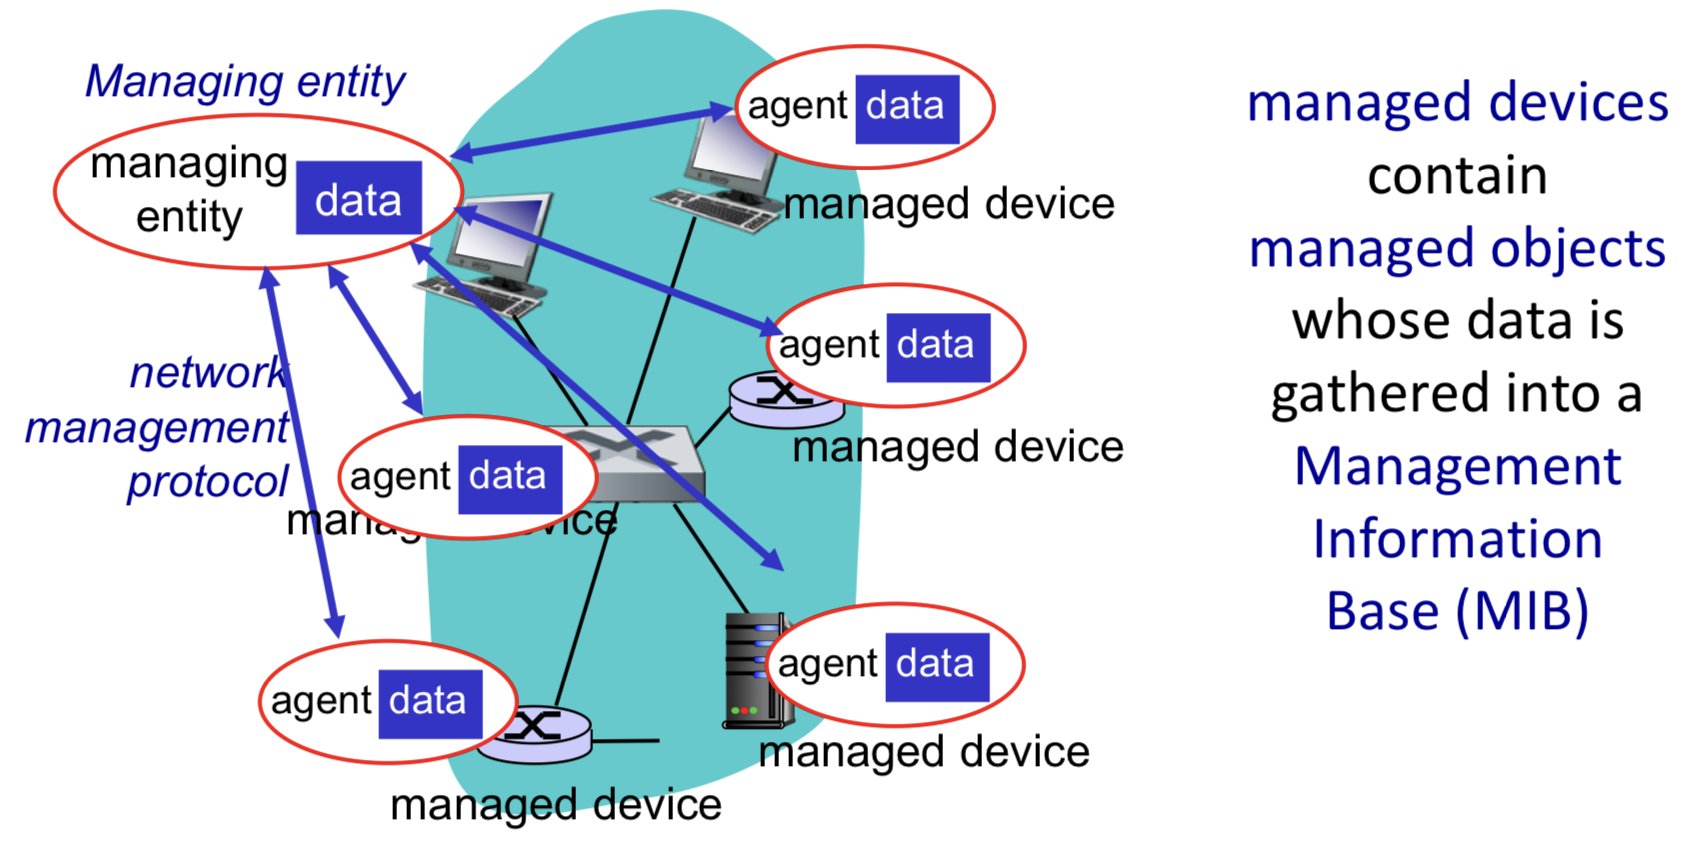
\includegraphics[width=0.75\textwidth]{img/SNMP.png}
\end{figure}

\subsubsection{Analisi dei componenti fondamentali di SNMP}

Per poter gestire una rete in modo efficace, è necessario definire in modo
preciso e non ambiguo quali dati raccogliere e come rappresentarli. SNMP
risolve questo problema attraverso due componenti strettamente correlati:
lo SMI e la MIB.

Lo SMI è un linguaggio di definizione dei dati il cui scopo è specificare la
sintassi e la semantica delle informazioni di gestione. SMI definisce un sottoinsieme 
di tipi di dati standard (esempio: INTEGER, OCTET STRING, Counter32) e due costrutti 
principali per organizzare le informazioni:

\begin{itemize}
\item \textbf{OBJECT-TYPE}: definisce un singolo oggetto gestito,
specificandone il tipo di dato, lo stato (esempio: corrente o obsoleto), i
permessi di accesso (esempio: sola lettura) e una descrizione testuale del
suo significato.
\item \textbf{MODULE-IDENTITY}: raggruppa un insieme di oggetti correlati in un
unico ``modulo MIB'', facilitando l'organizzazione e la gestione delle
informazioni.
\end{itemize}

La MIB è, di fatto, una collezione di oggetti gestiti, ognuno dei quali è
specificato formalmente tramite il costrutto OBJECT-TYPE dello SMI. Questi
oggetti rappresentano i dati di monitoraggio e vengono raccolti logicamente in
moduli. Ad esempio, un singolo oggetto potrebbe essere un contatore per i
``datagrammi entrati in uno schema di rete'', mentre un modulo MIB potrebbe
essere ``l'insieme di tutte le metriche e gli oggetti relativi al protocollo
IP''. Esistono centinaia di moduli MIB standardizzati, più un numero ancora
maggiore di moduli specifici dei vari produttori.

Per chiarire questi concetti, analizziamo due esempi pratici:

\begin{itemize}
\item \textbf{Esempio di oggetto: ipInDelivers}: questo oggetto, definito con
OBJECT-TYPE, ha una syntax di tipo Counter32 (un contatore a 32 bit che può
solo aumentare). Il suo MAX-ACCESS è \texttt{read-only}, indicando che può
solo essere letto ma non modificato. Lo STATUS è \texttt{current}, a
significare che è un oggetto valido e in uso. La DESCRIPTION chiarisce che
rappresenta il numero totale di datagrammi di input consegnati con successo
ai protocolli utente IP.
\item \textbf{Esempio di modulo: ipMIB}: questo modulo, definito con
MODULE-IDENTITY, raggruppa tutti gli oggetti relativi al protocollo IP. I suoi
campi forniscono metadati importanti, come LAST-UPDATED (data dell'ultimo
aggiornamento), ORGANIZATION (l'ente responsabile, in questo caso l'IETF),
CONTACT-INFO e una DESCRIPTION che ne riassume lo scopo.
\end{itemize}

\begin{figure}[H]
    \centering
    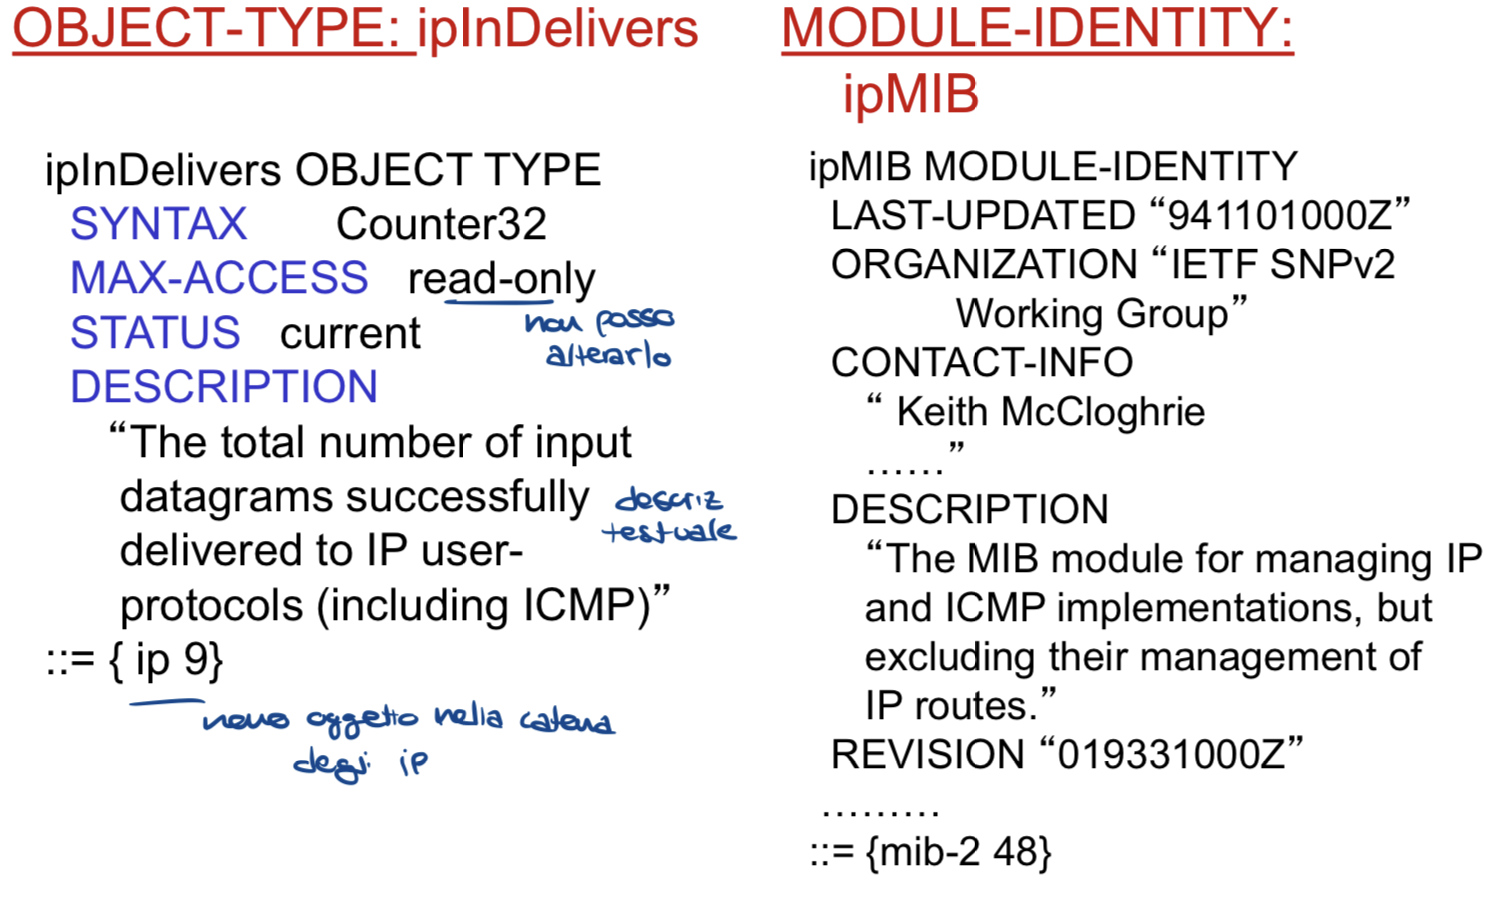
\includegraphics[width=0.75\textwidth]{img/SMI.png}
\end{figure}

Un esempio pratico di MIB è il modulo UDP, che contiene oggetti utili per
monitorare il protocollo. Oggetti come \texttt{UDPInDatagrams}
(datagrammi totali ricevuti) e \texttt{UDPOutDatagrams} (datagrammi totali
inviati) forniscono una visione generale del traffico, mentre
\texttt{UDPNoPorts} (datagrammi scartati per assenza di applicazioni in ascolto
sulla porta) e \texttt{UDPInErrors} (datagrammi scartati per altri motivi)
sono fondamentali per diagnosticare problemi di connettività.

\subsubsection{Il sistema di nomenclatura: l'albero OID}

Per assegnare un identificativo univoco standardizzato ad ogni oggetto 
è stato sviluppato l'\textbf{ISO Object Identifier (OID) Tree}, una
struttura gerarchica ad albero in cui ogni nodo ha sia un nome testuale che un
numero identificativo. Partendo da una radice comune (gestita dall'ISO), è
possibile navigare l'albero per raggiungere in modo univoco qualsiasi oggetto.
Ad esempio, l'OID \texttt{1.3.6.1.2.1.7.1} identifica in modo non ambiguo
l'oggetto \texttt{udpInDatagrams} seguendo il percorso:
\texttt{iso(1) $\to$ org(3) $\to$ dod(6) $\to$ internet(1) $\to$ mgmt(2)
$\to$ mib-2(1) $\to$ udp(7) $\to$ udpInDatagrams(1)}.

La struttura dell'albero OID è ben definita, con rami dedicati a diverse aree.
Sotto la radice \texttt{internet} troviamo il ramo \texttt{management}, che
contiene \texttt{mib-2}, il contenitore per i moduli MIB standardizzati più
comuni (system, interfaces, ip, tcp, udp, ecc.). Esiste anche un ramo
\texttt{private} utilizzato dai produttori per definire i propri oggetti
specifici, garantendo l'estensibilità del sistema.

\begin{figure}[H]
    \centering
    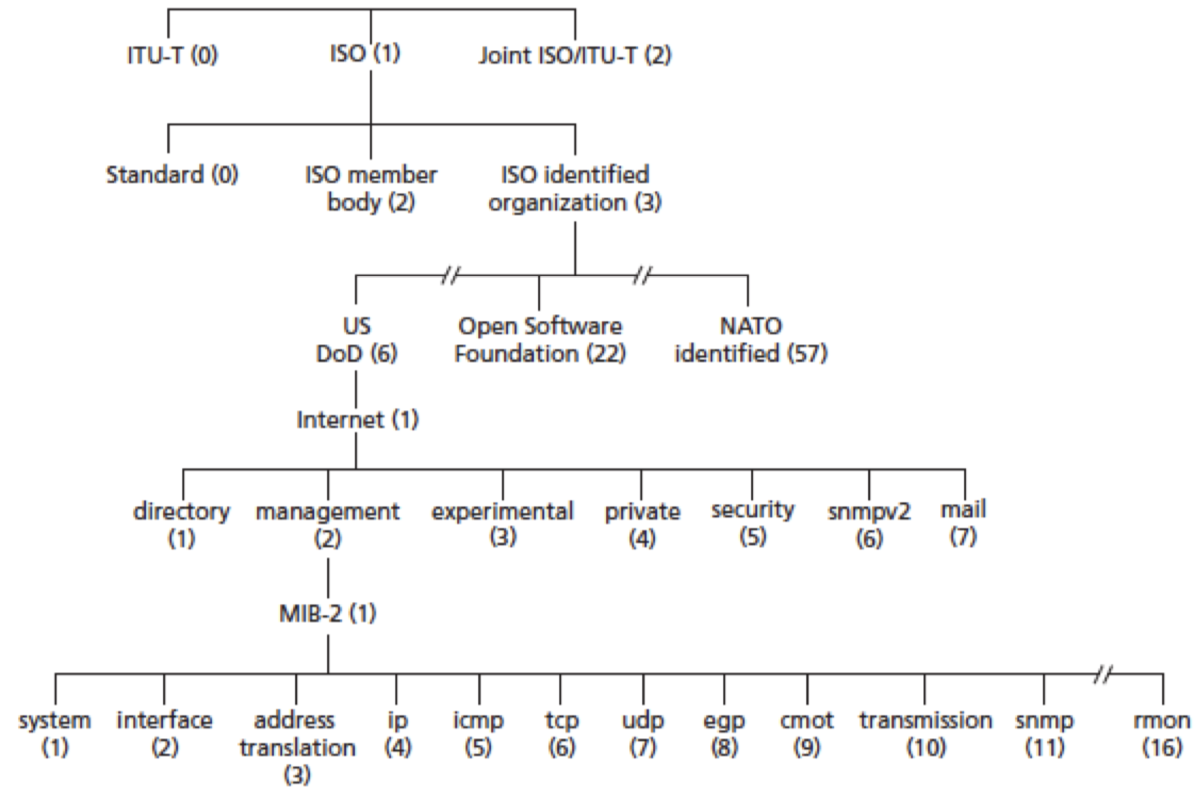
\includegraphics[width=0.75\textwidth]{img/tree.png}
\end{figure}

Analizziamo in dettaglio un oggetto fondamentale, \textbf{sysUpTime}:

\begin{itemize}
\item \textbf{Definizione}: OBJECT-TYPE con syntax TimeTicks (un contatore che
misura il tempo in centesimi di secondo).
\item \textbf{Accesso}: \texttt{read-only}.
\item \textbf{Stato}: \texttt{mandatory}, il che significa che la sua
implementazione è obbligatoria per ogni agente SNMP conforme allo standard.
\item \textbf{Descrizione}: ``Il tempo trascorso dall'ultima re-inizializzazione
della porzione di network management del sistema'', ovvero il tempo
trascorso dall'ultimo riavvio.
\item \textbf{OID}: \texttt{.1.3.6.1.2.1.1.3 ::= \{ system 3 \}}, 
che lo posiziona come terzo oggetto nel gruppo system.
\end{itemize}

\subsection{Il protocollo SNMP in azione}

\subsubsection{Modalità di comunicazione e messaggi}

Il protocollo SNMP definisce le regole per lo scambio di informazioni MIB tra
le entità di gestione e gli agenti sui dispositivi. Esistono due principali
modalità di interazione:

\begin{enumerate}
\item \textbf{Request/Response Mode}: la managing entity invia una richiesta
(esempio: per leggere un valore) e l'agent risponde con i dati richiesti.
Questo modello è ideale per il polling periodico e le interrogazioni mirate.
\item \textbf{Trap Mode}: l'agent può inviare spontaneamente una notifica
asincrona (un messaggio Trap) alla managing entity per segnalare un evento
eccezionale o il superamento di una soglia predefinita. Questa modalità è
conveniente quando la rete è grande o molto trafficata, poiché riduce il
carico del polling costante da parte del manager.
\end{enumerate}

Per implementare queste modalità, SNMP definisce diverse tipologie di messaggi:

\begin{itemize}
\item \textbf{Richieste di dati (da manager ad agent)}:
\begin{itemize}
\item \textbf{GetRequest}: richiede il valore di uno o più oggetti MIB
specifici.
\item \textbf{GetNextRequest}: richiede il valore dell'oggetto successivo a
quello specificato nell'albero MIB. È utile per ``scoprire'' la struttura di
una MIB o leggere tabelle intere.
\item \textbf{GetBulkRequest}: una richiesta massiva che permette di recuperare
una grande quantità di dati da una tabella MIB con una singola transazione,
ottimizzando la comunicazione.
\end{itemize}
\item \textbf{Operazioni di configurazione (da manager ad agent)}:
\begin{itemize}
\item \textbf{SetRequest}: utilizzato dalla managing entity per modificare il
valore di un oggetto MIB scrivibile su un dispositivo gestito.
\end{itemize}
\item \textbf{Risposte (da agent a manager)}:
\begin{itemize}
\item \textbf{Response}: messaggio inviato dall'agente in risposta a una
richiesta Get o Set, contenente i dati richiesti o la conferma
dell'operazione.
\end{itemize}
\item \textbf{Notifiche (da agent a manager)}:
\begin{itemize}
\item \textbf{Trap}: messaggio asincrono inviato dall'agente per notificare un
evento significativo.
\end{itemize}
\item \textbf{Comunicazione tra manager (da manager a manager)}:
\begin{itemize}
\item \textbf{InformRequest}: permette a una managing entity di inviare
informazioni da una MIB a un'altra, tipicamente in architetture di gestione
gerarchiche.
\end{itemize}
\end{itemize}

Il formato dei messaggi SNMP si differenzia in base alla funzione. I messaggi
di tipo richiesta/risposta (come Get, Set e Response) sono costruiti attorno a
campi per la gestione della transazione: \texttt{RequestID} per associare
risposte a richieste, \texttt{Error Status} per indicare eventuali errori ed
\texttt{Error Index} per specificare quale oggetto ha causato l'errore.
Al contrario, il messaggio Trap presenta un'intestazione distinta con campi come
\texttt{Enterprise} (che identifica chi ha definito il trap), \texttt{Agent Addr}
(l'indirizzo del mittente) e \texttt{Trap Type} per fornire un contesto immediato
sull'evento segnalato.

\subsection{Sicurezza in SNMPv3}

Le prime versioni di SNMP erano state progettate con la semplicità come obiettivo
primario, a scapito della sicurezza. Per risolvere questa grave lacuna,
SNMPv3 ha introdotto un'architettura di sicurezza modulare e robusta, basata su
meccanismi crittografici standard.

I principali meccanismi di sicurezza implementati in SNMPv3 sono:

\begin{itemize}
\item \textbf{Cifratura (Encryption)}: per garantire la riservatezza dei dati
di gestione, SNMPv3 supporta la cifratura dei messaggi. Lo standard prevede
l'uso dell'algoritmo DES (\textit{Data Encryption Standard}), basato su un
sistema a chiave simmetrica condivisa tra manager e agente.
\item \textbf{Autenticazione (Authentication)}: per garantire l'integrità del
messaggio e l'autenticità del mittente, SNMPv3 calcola un
\textit{Message Integrity Code} (MIC), utilizzando una funzione di hashing
applicata al messaggio insieme a una chiave segreta condivisa.
\item \textbf{Protezione contro il replay (Playback Protection)}: per prevenire
attacchi in cui un aggressore cattura un messaggio valido e lo reinvia in un
secondo momento, SNMPv3 utilizza un meccanismo di \textit{nonce}. Questo
valore si basa su un contatore che riflette il tempo trascorso dall'ultimo
riavvio del software di gestione, garantendo che ogni messaggio sia unico e
impedendo che un messaggio obsoleto venga accettato come valido.
\item \textbf{Controllo degli accessi (View-Based Access Control)}: SNMPv3
permette di definire policy con un database che specifica i diritti 
di accesso per utenti diversi, limitando non solo quali operazioni possono 
eseguire (lettura, scrittura) ma anche quali porzioni dell'albero MIB
possono accedere.
\end{itemize}

L'architettura di SNMPv3 riflette questa modularità. Una PDU
(\textit{Protocol Data Unit}) generata da un'applicazione SNMP passa attraverso
uno SNMP engine. Qui, il sottosistema di Message Processing la elabora e la
passa al modulo di sicurezza, che applica i servizi richiesti: Timeliness
(protezione dal replay), autenticazione e privacy (cifratura). Infine, la PDU
viene incapsulata in un header di sicurezza e inviata sul livello di trasporto.

Questo approccio stratificato ha reso SNMP un protocollo adatto anche alla 
gestione di infrastrutture critiche. 
Oltre alla sicurezza un altro problema fondamentale nella comunicazione tra 
sistemi eterogenei è la presentazione dei dati.

\subsection{Il problema della presentazione dei dati e la soluzione ASN.1}

Anche con un protocollo ben definito, la comunicazione tra due sistemi può
fallire se questi utilizzano formati di dati interni diversi. Il cosiddetto
``problema della presentazione'' sorge perché una semplice copia
\textit{memory-to-memory} dei dati non è sufficiente quando le architetture
degli host differiscono, ad esempio per l'ordine dei byte (\textit{byte order}).
Una struttura che contiene il valore intero 256 può essere memorizzata in modi
diversi su due host, rendendo i dati incomprensibili se trasferiti direttamente.

Esistono tre approcci per risolvere questo problema:
\begin{enumerate}
\item Il mittente impara il formato del destinatario e traduce i dati prima di
inviarli. Questo approccio non è scalabile in una rete con molti sistemi
diversi (\(N \cdot (N-1)\) traduttori necessari).
\item Il mittente invia i dati nel suo formato nativo e il destinatario si
occupa della traduzione. Anche questo non è scalabile.
\item Il mittente e il destinatario si accordano su un \textbf{formato
intermedio indipendente dall'host}. Il mittente traduce dal suo formato nativo
a quello intermedio, e il destinatario traduce dal formato intermedio al
proprio. Questa è la soluzione più efficiente e scalabile.
\end{enumerate}

La soluzione standard adottata nel mondo delle reti è \textbf{ASN.1}
(\textit{Abstract Syntax Notation One}), uno standard ISO che permette
di definire i tipi di dati e le strutture in modo indipendente dalla piattaforma.
ASN.1 definisce la sintassi astratta, mentre le \textbf{BER}
(\textit{Basic Encoding Rules}) specificano come gli oggetti definiti in ASN.1
debbano essere codificati per la trasmissione.

Le BER utilizzano una codifica \textbf{TLV}, in cui ogni dato è rappresentato 
da tre campi:
\begin{itemize}
\item \textbf{T (Type)}: un codice che caratterizza il tipo di dato
(esempio: INTEGER, OCTET STRING).
\item \textbf{L (Length)}: la lunghezza in byte del campo valore.
\item \textbf{V (Value)}: il valore effettivo del dato, codificato secondo le
regole standard.
\end{itemize}

Grazie a questa tecnica, un ricevitore può sempre interpretare correttamente il
flusso di byte ricevuto: dopo aver letto il tipo e la lunghezza, sa esattamente
quanti byte successivi costituiscono il valore, anche senza conoscere a priori
la struttura esatta del messaggio.

\subsection{Evoluzione delle soluzioni di gestione della rete}

SNMP ha giocato un ruolo fondamentale come protocollo storico per il monitoraggio
e la gestione delle reti, e rimane ampiamente utilizzato, specialmente per la
raccolta di dati prestazionali. Tuttavia, per compiti più complessi come la
gestione delle configurazioni su larga scala, sono emerse soluzioni più moderne
e potenti che ne estendono o sostituiscono le funzionalità.

L'evoluzione della gestione di rete si è mossa verso paradigmi basati su modelli
di dati strutturati e API di tipo web. Le tecnologie chiave in questo ambito sono:

\begin{itemize}
\item \textbf{NETCONF e RESTCONF}: protocolli progettati specificamente per la
gestione della configurazione dei dispositivi di rete.
\item \textbf{YANG}: un linguaggio di modellazione dei dati utilizzato per
definire la struttura dei dati di configurazione e operativi, nonché le
operazioni RPC (\textit{Remote Procedure Call}) implementate dai dispositivi.
\item \textbf{Formati dati moderni}: utilizzo di formati leggibili come YAML,
JSON o XML per la rappresentazione dei dati, in sostituzione della codifica
binaria di SNMP.
\end{itemize}

In particolare, NETCONF opera tra un server di gestione e i dispositivi di rete,
utilizzando un paradigma chiamato \textit{Remote Procedure Call} (RPC).
Le sue funzionalità principali includono:
\begin{itemize}
\item Recuperare, impostare, modificare e attivare configurazioni.
\item Eseguire commit atomici di configurazioni su più dispositivi,
garantendo la coerenza.
\item Interrogare dati operativi e statistiche in tempo reale.
\item Sottoscrivere e ricevere notifiche di eventi dai dispositivi.
\end{itemize}

L'architettura di NETCONF è stratificata: i messaggi RPC, codificati in XML,
vengono scambiati su un canale di trasporto sicuro e affidabile (come TLS) 
per eseguire operazioni sulla configurazione del
dispositivo o per ricevere notifiche di eventi. Questo approccio basato su
modelli dati espliciti e transazioni robuste rappresenta il futuro della gestione
automatizzata e programmabile delle reti.

Un'alternativa a NETCONF è RESTCONF, basata su API REST. Invece di
invocare funzioni da remoto (come in RPC), utilizza le funzioni messe a
disposizione dalle API. Inoltre, al posto di XML è possibile utilizzare
YAML/JSON, che risultano più snelli e semplici.

\subsection{Problemi aperti e direzioni future}

\subsubsection{Problemi aperti}

Sia NETCONF sia SNMP presentano due limiti principali:

\begin{itemize}
\item \textbf{Misure passive}: possono solo collezionare statistiche aggregate
sullo stato dei dispositivi, senza alterare il traffico aggiungendo informazioni.
Ad esempio, è possibile aggregare le statistiche per protocollo (TCP, UDP,
\ldots) oppure per interfaccia.
\item \textbf{Scala temporale}: lavorano su scale temporali dell'ordine del
secondo o del minuto, troppo lente per alcuni fenomeni di rete.
\end{itemize}

È possibile cercare di rimediare a tali limiti utilizzando tre strumenti di
misura attiva:

\begin{itemize}
\item \textbf{Ping}: permette di stimare lo stato dei dispositivi e la latenza.
\item \textbf{Traceroute}: permette di tracciare il percorso di un protocollo
nella rete, sfruttando il campo TTL.
\item \textbf{NMAP}: permette di effettuare uno scan, ovvero scoprire quali
porte del livello 4 sono attive in un host (quelle su cui c'è un processo in
ascolto).
\end{itemize}

Nonostante si tratti di misure attive, le tre tecniche precedentemente elencate
hanno una portata informativa limitata.

\subsubsection{Direzioni future}

Le tecniche passive sono basate sulla cattura e l'analisi del traffico. Gli
strumenti più popolari per fare ciò sono tcp-dump e Wireshark. Tali strumenti
non sono però dedicati ai controlli continui. Per farlo è infatti necessario il
concetto di flusso (sequenza di pacchetti IP che condividono attributi comuni
come indirizzo IP/porta mittente-destinatario, protocollo, numero di byte
trasmessi, \ldots).

Esistono due approcci:

\begin{itemize}
\item \textbf{NetFlow}: basato sull'esportazione di informazioni aggregate per
il singolo flusso. I flussi possono essere TCP e UDP (nel caso UDP si usano
indirizzi e porte mittente/destinatario per identificarli).
\item \textbf{sFlow}: prevede un campionamento del flusso da inviare a una
stazione di monitoraggio.
\end{itemize}

NetFlow e sFlow rappresentano misure passive. Per quanto riguarda invece le
misure attive, esiste un nuovo framework chiamato \textbf{telemetria di rete},
che prevede che i nodi giochino un ruolo attivo: mentre inviano traffico,
aggiungono e rimuovono intestazioni. Si tratta di misure attive perché non si
limitano a osservare il traffico, ma lo modificano attraverso l'aggiunta di
intestazioni. Le modalità attive prevedono l'uso della CPU.

SNMP resta comunque una valida soluzione per le misurazioni della banda:
permette infatti di effettuare monitoraggi sul lungo periodo.

\begin{figure}[H]
    \centering
    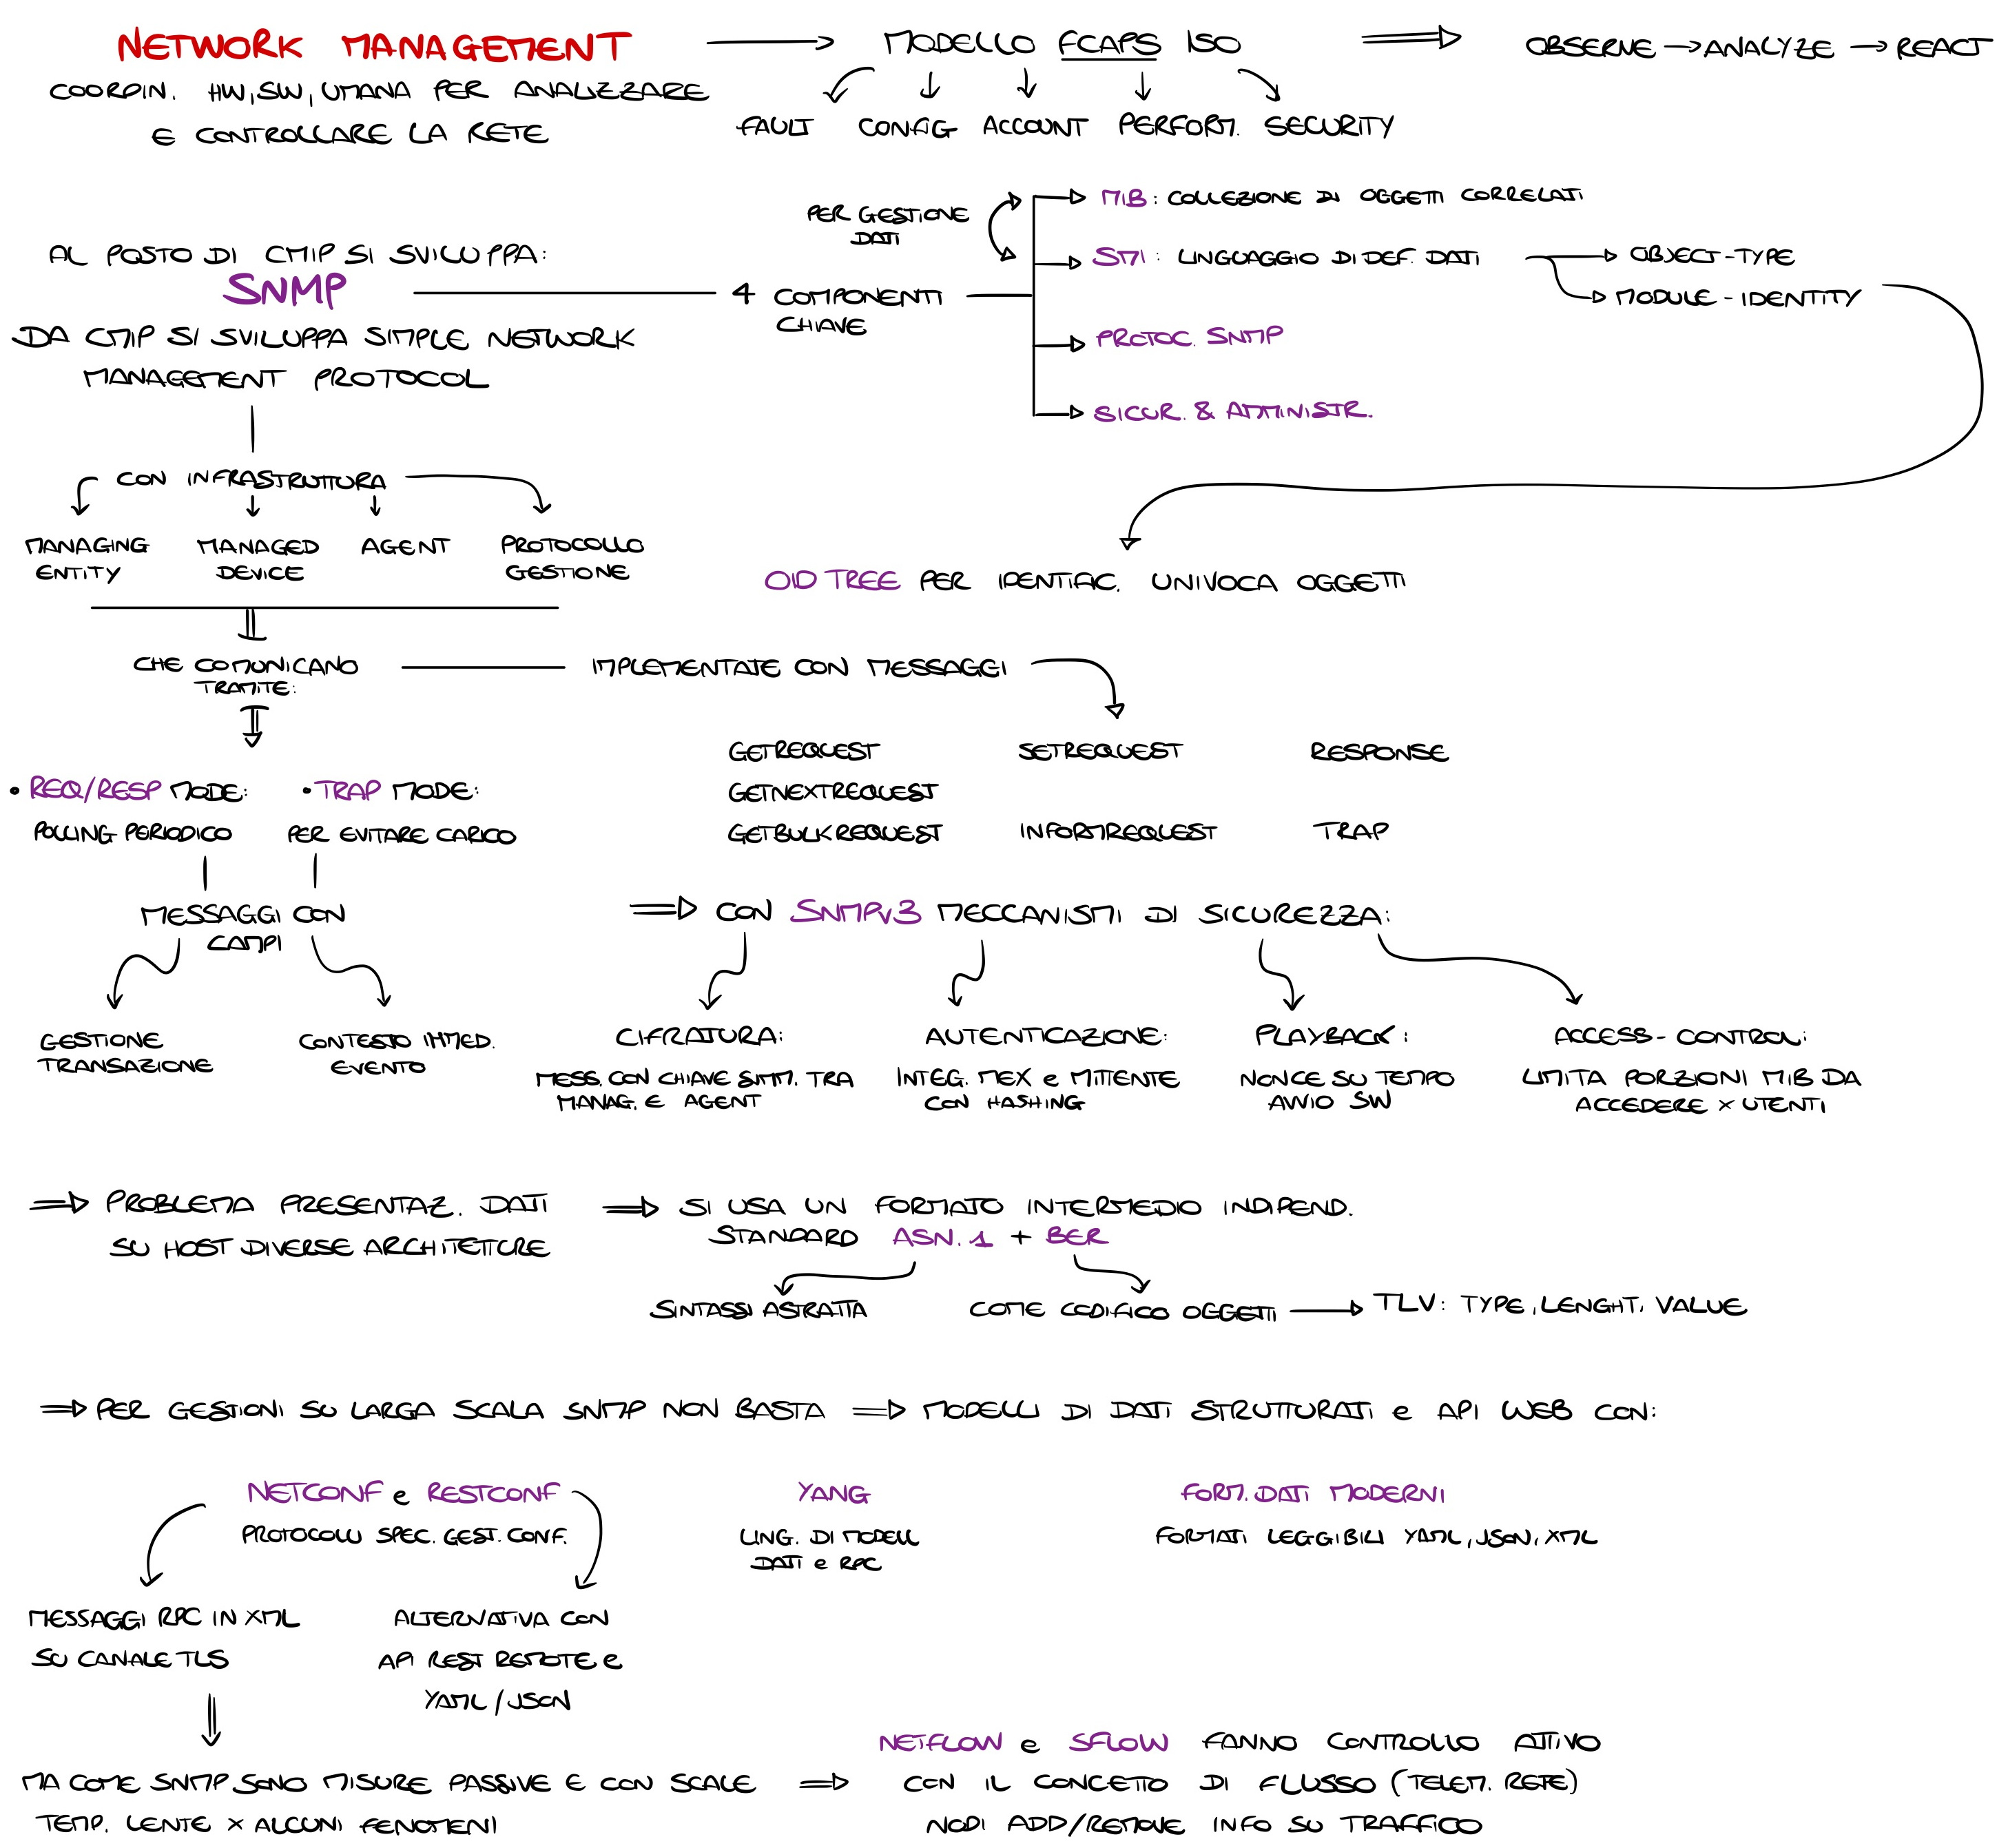
\includegraphics[width=1\textwidth]{img/1.jpg}
    \caption*{Schema capitolo 1}
\end{figure}